\section{Operators between TFSM and Activity}
	\begin{itemize}
		\item \todo{To show only the hierarchical coordination!}
		\item \todo{This example has to show the benefice of our approach in term of automatic coordination and variations of the semantics of the coordination}
		\item \todo{The no timing hierarchical coordination must be specify in one operator by relying on a library}
			
		\item Operator captures a given coordination pattern between TFSM and the fUML language
		\item We capture a timing and hierarchical coordination pattern.
		\item We use these operators to coordinate a surveillance camera system (Moto)
		\item We verify and verify the coordinated system.

	\end{itemize}
	
	
	\subsection{Definition}
	
	In a \bcool specification (see Listing~\ref{fig:bcoolsyncrohetero}: line 1), we define four coordination operators between the TFSM and fUML languages. The specification begins by importing (see Listing~\ref{fig:bcoolsyncrohetero}: line 3 and 4) the behavioral interfaces of each language, defined as an \ecl specification.
	
	
	\todo{The first operator, named \emph{SyncProduct} (see Listing~\ref{fig:bcoolsyncrohetero}: line 6), differs from the running example because it applies to heterogeneous languages (namely fUML and TFSM). 
	Whereas in the running example the occurrences of FSMEvents were synchronized with the occurrences of other FSMEvents, here they are synchronized with the start of fUML \emph{Actions}, \ie by coordinating instances of \dse \emph{occurs} and \emph{startAction}.} 

	For the second and third operators, we specify a hierarchical coordination pattern between the TFSM and fUML languages, unlike hierarchical coordination frameworks where the semantics is hidden, these operators explicitly specify how the hierarchical coordination is implemented. In our case, we chose the semantics in which entering a specific state of a TFSM model triggers the execution of a given fUML activity. When leaving a state, several semantic variation points may be chosen. The outgoing transitions from a state can be considered, for instance, as preemptive for the activity model (\ie firing a transition from a state to another preempts the internal activity). Alternatively, the transition can be considered as non-preemptive (\ie the states cannot be left before the associated activity finishes). In this paper, we chose non-preemptive transitions, preemptive ones are detailed on the companion webpage. Listing~\ref{fig:bcoolnopremtive} presents the \bcool specification that is organized around two operators: \textit{StateEntering} and \textit{StateLeaving}. 
	
	\begin{lstlisting}[language=bcool,
	caption={Heterogeneous synchronized product operator between the TFSM and fUML languages},
	label={fig:bcoolsyncrohetero}, 
	basicstyle=\scriptsize\ttfamily, backgroundcolor=\color{LGrey}, numbers=left, xleftmargin=2pt]
	BCOoLSpec TFSM-fUMLOperators
	ImportLib "facilities.bcoollib"
	ImportInterface "activitySemantics.ecl" as activity
	ImportInterface "TFSM.ecl" as tfsm
	
	Operator SyncProduct(dse1 : activity::startAction, dse2 : tfsm::occurs)
	CorrespondenceMatching: when(dse1.name = dse2.name)
	CoordinationRule: RendezVous(dse1, dse2)
	end operator
	\end{lstlisting}
	
	
	
	\begin{lstlisting}[language=bcool,
	caption={Hierarchical coordination operators between TFSM and fUML languages},
	label={fig:bcoolnopremtive}, 
	basicstyle=\scriptsize\ttfamily, backgroundcolor=\color{LGrey}, numbers=left,firstnumber=10, xleftmargin=2pt]
	Operator StateEntering(dse1 : activity::startActivity, dse2 : tfsm::entering)
	CorrespondenceMatching: 
	when(dse1.name = dse2.onEnterAction.name)
	CoordinationRule: RendezVous(dse1, dse2)
	end operator
	
	Operator StateLeaving(dse1 : activity::finishActivity, dse2 : tfsm::leaving)
	CorrespondenceMatching: 
	when(dse1.name = dse2.onEnterAction.name)
	CoordinationRule: Causality(dse1, dse2)
	end operator
	
	\end{lstlisting}
	
	For the fourth operator, we deal with the temporal aspects of the model coordination. The operator specifies how the time in the TFSM elapses during the execution of the activities that specify the on-entry action of a state. This coordination is also hierarchical, but in this case, only considers the timing aspects. In the TFSM language, each state machine has a \emph{localClock} used to measure the time (see Figure~\ref{fig:tfsmmm}) while the fUML language is untimed. The local clock is a \emph{FSMClock}, which defines a \dse named \emph{ticks} whose occurrences represent a physical time increment. In the fUML language, the duration of activities can be represented as the time between the \dse \emph{startActivity} and \dse \emph{finishActivity} (Listing~\ref{fig:eclfuml}). To coordinate the time, it is necessary to specify the number of \emph{ticks} of the local clock between the occurrence of the \dse \emph{startActivity} and \emph{finishActivity}. We propose an operator that enforces the execution of the ``internal'' activity to be atomic with respect to the time in the TFSM model. As a result, there is no occurrence of the \dse ticks of the corresponding local clock during the execution of the activity. 
	
	Listing~\ref{fig:bcooltimeinactions} captures the corresponding coordination pattern by defining the operator named \emph{NoTimeinRefinedActivity}. The operator selects instances of \dse startActivity and finishActivity by using their context. As a result, the pairs selected identify the starting and finishing of an activity. Then, we select the activities that represent a state (Listing~\ref{fig:bcooltimeinactions}: line 24). To do so, we use the onEnterAction defined in the context of State. Then, we use the selected instances of \dse entering to select instances of \dse ticks of the corresponding local clock (Listing~\ref{fig:bcooltimeinactions}: line 25). The coordination rule must specify how much time is consumed during the execution of an activity. First, we use the event expression \emph{SampledBy} to create a local event named \emph{sampled} which ticks always after the startActivity instance, and coincides with the occurrences of the instance of the corresponding \dse ticks (Listing~\ref{fig:bcooltimeinactions}: line 27). Second, we synchronize the event sampled with the finishing of the activity by using a causality relation (Listing~\ref{fig:bcooltimeinactions}: line 28). This results for instances of ticks to occur only after the activity has finished its execution.
	
	The coordination rule presented earlier can be built by relying on a \bcool library. In this case, we have to extend the library \emph{facilities.bcoollib} and add a new event relation named \emph{atomicActivity}. Then, we have to replace the event expressions and relations by the event relation atomicActivity with the corresponding parameters (\ie dse1, dse2, dse4). The use of the library to define domain specific relations has two major benefits. First, once defined in the library, event relations can be reused in various \bcool specifications. Second, by defining a dedicated event relation, we improve the readability and modularity of the \bcool specification.
	
	\begin{lstlisting}[language=bcool,
	caption={Timing coordination operator between TFSM and fUML language},
	label={fig:bcooltimeinactions}, 
	basicstyle=\scriptsize\ttfamily, backgroundcolor=\color{LGrey}, numbers=left,firstnumber=21, xleftmargin=2pt, aboveskip=3pt] 
	Operator NoTimeinRefinedActivity(dse1 : activity::startActivity, dse2 : activity::finishActivity, dse3 : tfsm::entering, dse4 : tfsm::ticks)
	CorrespondenceMatching:
	when (dse1.name = dse2.name)
	and  (dse1.name = dse3.onEnterAction.name)
	and  (dse3.owningFSM.localClock = dse4)
	CoordinationRule:
	Local Event sampled = SampledBy(dse1, dse4);
	Causality(dse2, sampled)
	end operator	 
	\end{lstlisting}
	
	\subsection{Use of the Operators in a Surveillance Camera System}
	In this section, we develop the heterogeneous model of a surveillance camera system (see Figure~\ref{fig:camerasystem}). To model different aspects of the system, we use the TFSM and the fUML languages. Then, we use the operators developed in the previous section to generate the coordination specification. 
	
	The video surveillance system is composed of a camera and a battery control. The camera takes pictures by using either the \emph{JPEG2000} or \emph{JPG} algorithm and is powered by a battery. When the battery is low, the battery control makes the camera use the \emph{JPG} algorithm, thus reducing the quality of the picture but also the energy consumption~\cite{encodingcomparison}. When the battery is high, the JPEG2000 algorithm is used instead. In Figure~\ref{fig:camerasystem}, the activity diagrams named \emph{BatteryControl} represents the simple algorithm implemented in the battery control. At the bottom of Figure~\ref{fig:camerasystem}, the TFSM named \emph{CameraControl} represents a partial view of the camera. When the TFSM model is in state \emph{BatteryHigh}, the JPEG2000 algorithm is used (specified by the activity diagram on the right of Figure~\ref{fig:camerasystem} named \emph{doJPEG2000}). When in state \emph{BatteryLow}, the encoding algorithm is replaced by a mere JPEG algorithm represented by an activity named \emph{doJPEG} (The activity is not shown for lack of space). The transition from one state to another is done when either the \emph{BatteryIsHigh} event or the \emph{BatteryIsLow} event occurs, depending on the current state.	 
	
	\begin{figure}
		\center
		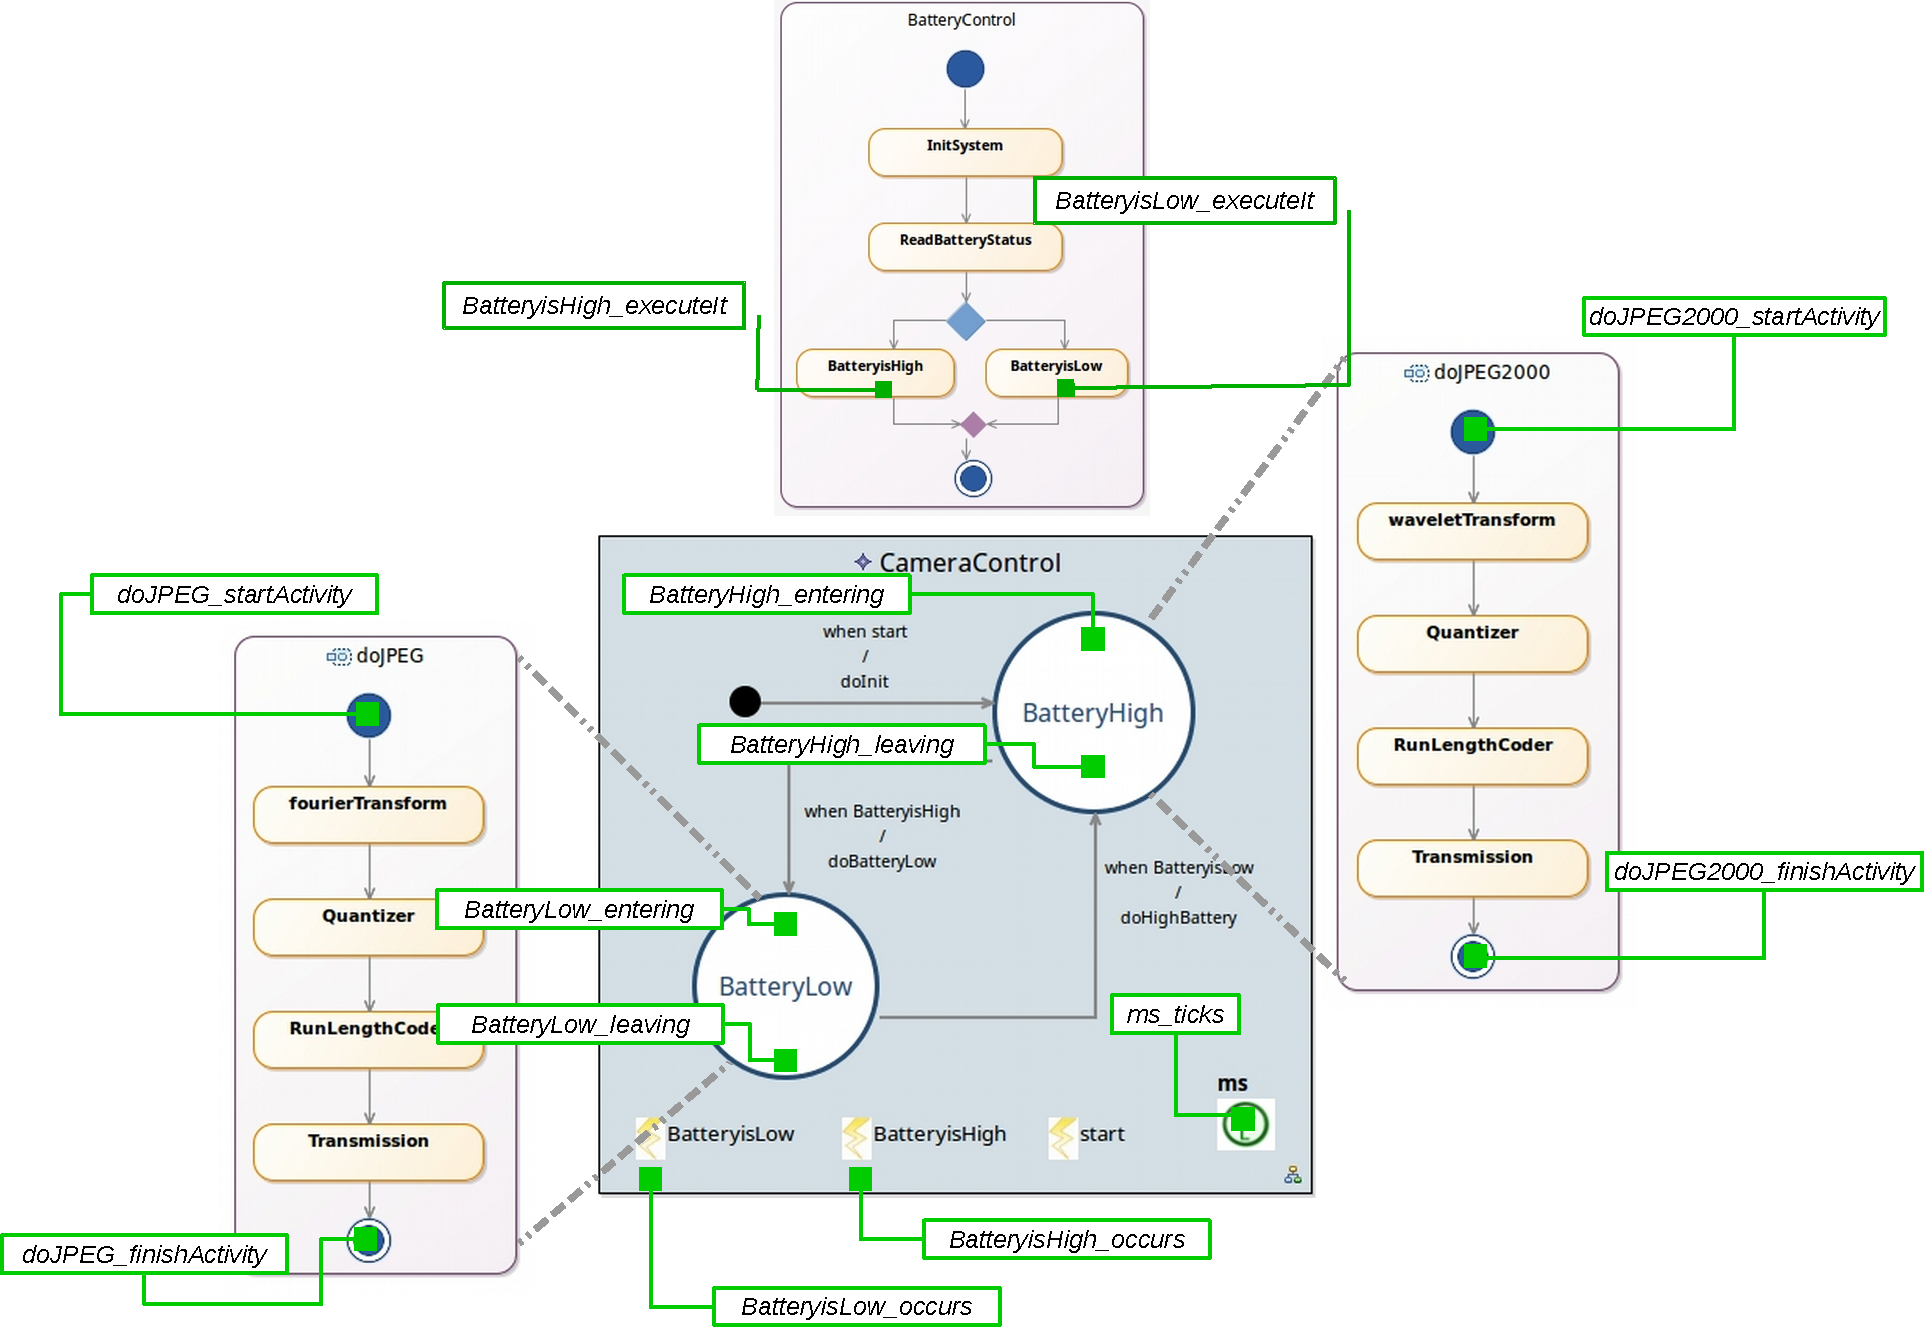
\includegraphics[width=.6\columnwidth]{examples/figs/picmodels.pdf}
		\caption{Hierarchical model of a surveillance camera system and a partial representation of the behavioral interface}
		\label{fig:camerasystem}
	\end{figure}
	
	To coordinate the models, we have to specify a timing and hierarchical coordination between the states of the TFSM CameraControl and the activities doJPEG and doJPEG2000. In addition, we have to synchronize the activity BatteryControl and the TFSM CameraControl by coordinating the corresponding Action and FSMEvent. Applying the four operators on these simple models, we generate the expected coordination specification. The coordination generated by using our approach corresponds to eight \ccsl relations.
	 
	In \bcool, the generated coordination specification conforms to the CCSL language. Since we are using a formal language, the integrator can execute and verify the coordination specification of the system.
	
	By using the language workbench presented in Section~\ref{section:bcoollengbench}, the coordination specification generated for the surveillance camera system can be executed and analysed. More precisely, we are able to execute the coordination specification by using TimeSquare, and to explore the state space. For lack of space we do not show the timing output of the execution of the surveillance camera system, however, the models together with a procedure to execute and verify them can be found in the companion web site.
	
	\todo{to show a timing and state space exploration}
	\subsection{Discussion}
	
	\begin{itemize}
		\item Discussion by relying on the criteria presented in evaluation.
		\item Semantics variation of the hierarchical coordination. 
		\item automatic generation of the coordination, eight relation.
		\item Verification and validation. 
	\end{itemize}